\PassOptionsToPackage{dvipsnames}{xcolor}
\documentclass[
    a5paper,
    spinewidth=10mm,
    markcolor=black,
    %trimmed % Show only trimmed part!
    ]{bookcover}

% \bookcovertrimmedpart{front} % Trimmed part is the front cover
% \bookcovertrimmedpart{back} % Trimmed part is the back cover
% \bookcovertrimmedpart{spine} % Trimmed part is the spine 

\usepackage{fix-cm}
\usepackage[latin]{babel}
\usepackage{lipsum,microtype,GS1,qrcode}

% Couleurs personnalisées et graphiques TikZ
\usepackage[dvipsnames]{xcolor}
\usepackage{graphicx}
\usepackage{tikz}
\usetikzlibrary{calc}
\begin{document}

\begin{bookcover}


    \bookcovercomponent{normal}{front}{
        \begin{tikzpicture}[overlay,remember picture]
            \node[inner sep=0pt, anchor=north east] at ($(current page.north east)-(1.2cm,1cm)$) {
                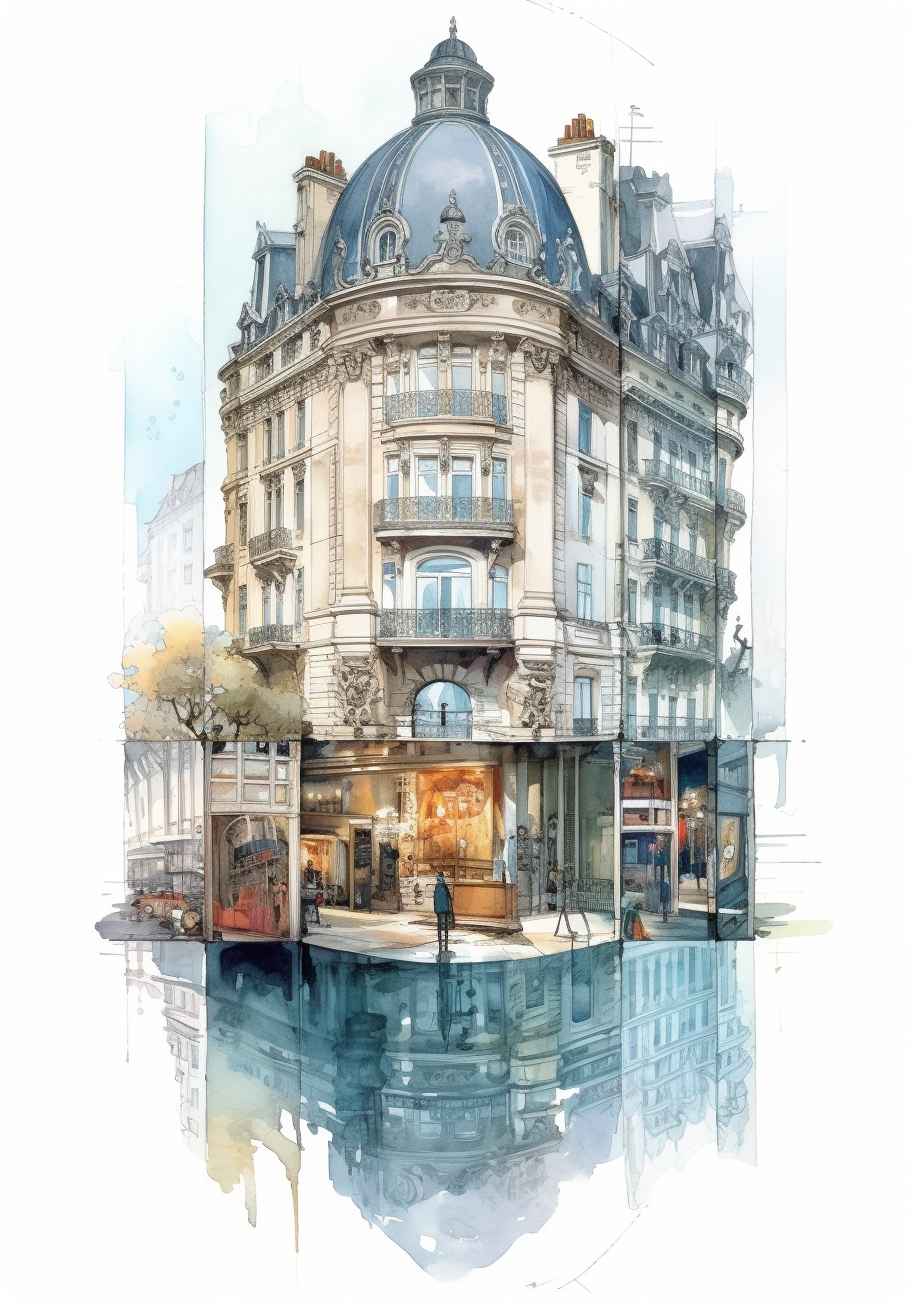
\includegraphics[width=172mm, keepaspectratio]{images/375669df-73f6-4168-9295-19bef29746b5.png}
            };

            % White frame with 0.33 opacity
            \fill[white, opacity=0.33] (current page.south west) rectangle (current page.south east |- current page.center);

            % Title
            \node[align=center] at ($(current page.north east)-(9.6cm,19.5cm)$)
            {
            {\fontsize{45}{72} \fontfamily{cmr}\selectfont \textcolor{black}{\textbf{L'envers du décor}}}\\[0.5cm]
            {\fontsize{30}{72} \fontfamily{cmr}\selectfont \textcolor{black}{\textbf{des Entreprises}}}\\[0.25cm]
            {\fontsize{45}{72} \fontfamily{cmr}\selectfont \textcolor{black}{\textbf{Libérées}}}
            };

            % Author
            % Author
            \node[align=center] at ($(current page.south east)+(-10,2)$)
            {
                {\fontsize{12}{19.2} \textcolor{black}{\selectfont {Kevin Delfour}}}\\[3pt]
            };

        \end{tikzpicture}
    }

    \bookcovercomponent{normal}{spine}[3mm,5mm,5mm,3mm]{
        \rotatebox[origin=c]{-90}{
            \fontfamily{cmr}
            \textbf{L'envers du décor des Entreprises Libérées}
        }
        \vfill
        \rotatebox[origin=c]{-90}{
            \fontfamily{cmr} Kevin Delfour
        }
    }

    \bookcovercomponent{normal}{back}[22mm,10mm,22mm,30mm]{
        \begin{tikzpicture}[overlay,remember picture]
            \node[align=left, text width=120mm] at ($(current page.north)-(9.6cm,7.5cm)$)
            {
                {\fontsize{25}{72} \fontfamily{cmr}\selectfont \textcolor{black}{\textbf{L'envers du décor des Entreprises Libérées}}}\\[0.5cm]

                \fontsize{12}{15} \fontfamily{cmr}\selectfont \textcolor{black}{Dans un monde où les structures d'entreprise traditionnelles rencontrent de plus en plus de défis, le modèle d'entreprise libérée émerge comme une solution prometteuse, mais complexe.}\\[0.15cm]

                \fontsize{12}{15} \fontfamily{cmr}\selectfont \textcolor{black}{Plongeant dans l'envers du décor des entreprises libérées, explorant l'équilibre délicat entre autonomie et cohésion, et abordant des sujets cruciaux tels que le recrutement, l'intégration, la formation et le développement des compétences, ce guide éclaire les mythes et réalités, offre des conseils pratiques, et invite le lecteur à une réflexion profonde sur ce que signifie vraiment "libérer" une entreprise.}
            };

            \node[align=left, text width=120mm] at ($(current page.center)-(9.6cm,2.5cm)$)
            {
                {\fontsize{25}{72} \fontfamily{cmr}\selectfont \textcolor{black}{
                            \textbf{À propos de l'auteur}
                        }}\\[0.5cm]

                \fontsize{12}{15} \fontfamily{cmr}\selectfont \textcolor{black}{
                    Kevin Delfour, développeur logiciel expérimenté, est passionné par l'innovation et l'holacratie. Il a réorienté sa carrière pour devenir responsable d'une société de service, construite sur le modèle d'Entreprise Libérée. Il vise à rendre les entreprises plus agiles et réactives aux changements grâce à l'innovation.
                }\\[0.25cm]
            };

        \end{tikzpicture}
    }

    \bookcovercomponent{normal}{back}[,1cm,,]{
        \vfill
        \centering
        \small{\textcolor{darkgray}{ISBN: 000-00-000-0000-0}}\\
        \small{\textcolor{darkgray}{Edition \textbf{{Le Vilain Petit Dev}}}}\\[0.5cm]

        \savebox0{
            \EANBarcode[module_height=15mm]{ISBN 000-00-000-0000-0}
        }
        \colorbox{white}{
            \usebox0
        }
    }

    %\bookcovercomponent{ruler}{whole}{,,} % Check dimensions

\end{bookcover}

\end{document}